\def\secforfig{appendices/vbfbkgd-shifted-region}
\def\figsversion{V2}

\begin{figure}[ht]
    \centering
    \subfloat[${\pt}_{2}$]{%
            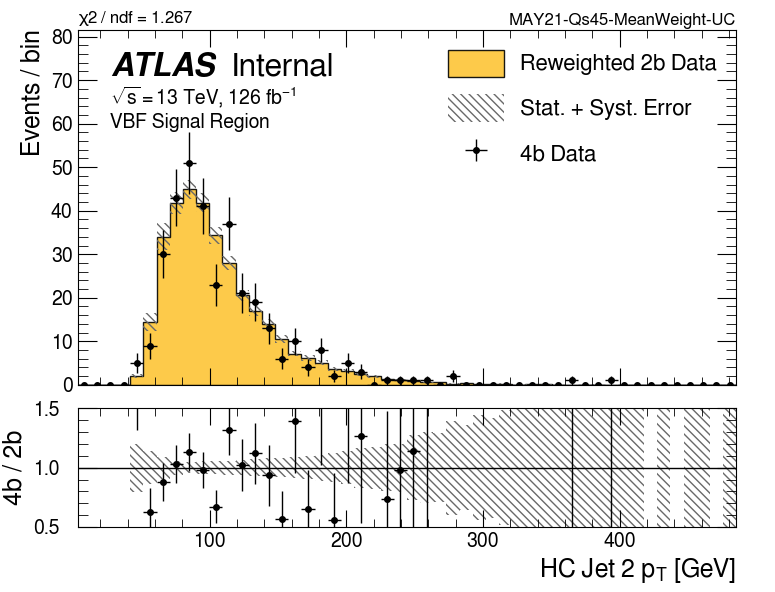
\includegraphics[width=0.25\textwidth]{\figpath{upper-center/sig/ALL/MAY21-Qs45-MeanWeight-UC-pT-2-Signal-Region-NN-all-4bvbfinclusive.png}}
    }
    \subfloat[${\pt}_{4}$]{%
            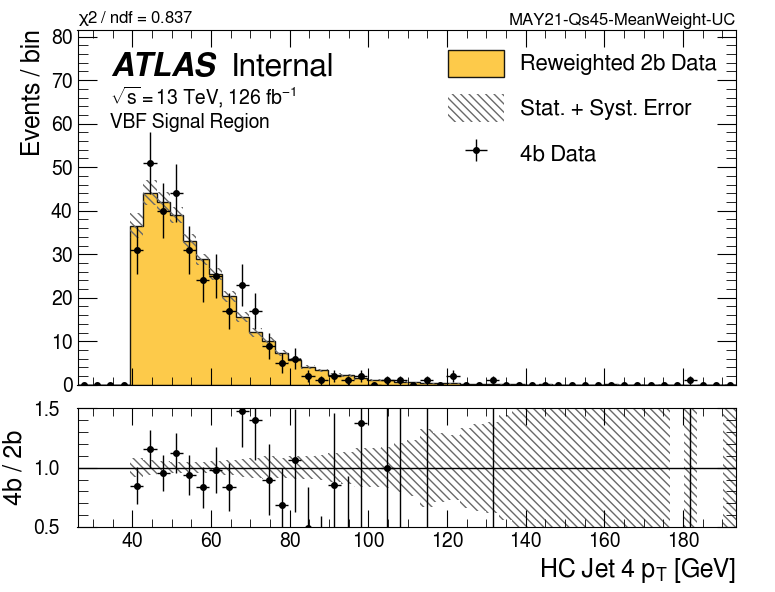
\includegraphics[width=0.25\textwidth]{\figpath{upper-center/sig/ALL/MAY21-Qs45-MeanWeight-UC-pT-4-Signal-Region-NN-all-4bvbfinclusive.png}}
    }
    \subfloat[$dR_{jj,1}$]{%
            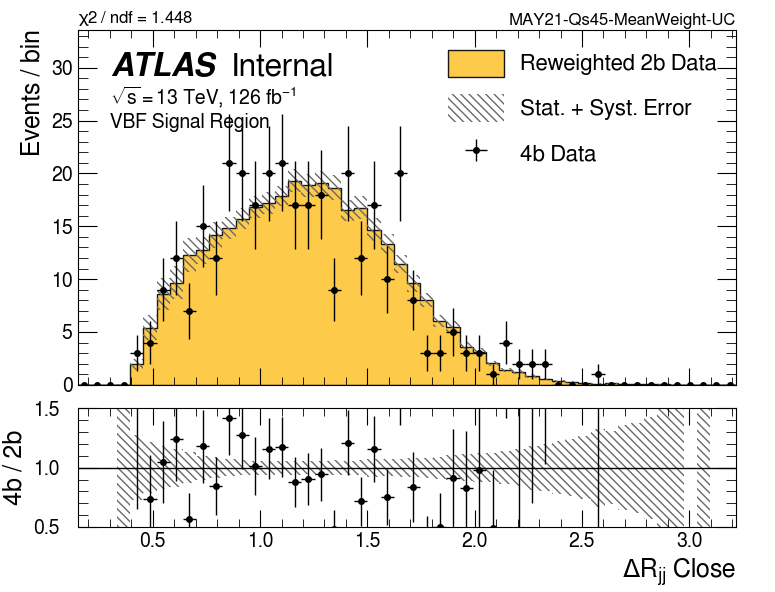
\includegraphics[width=0.25\textwidth]{\figpath{upper-center/sig/ALL/MAY21-Qs45-MeanWeight-UC-dRjj-1-Signal-Region-NN-all-4bvbfinclusive.png}}
    }
    \subfloat[$dR_{jj,2}$]{%
            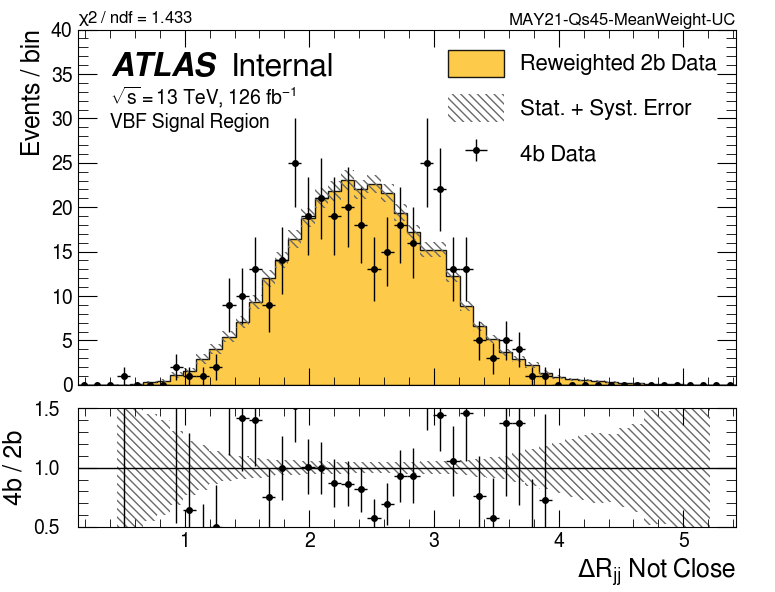
\includegraphics[width=0.25\textwidth]{\figpath{upper-center/sig/ALL/MAY21-Qs45-MeanWeight-UC-dRjj-2-Signal-Region-NN-all-4bvbfinclusive.png}}
    }

    \subfloat[$\eta_{i}$]{%
            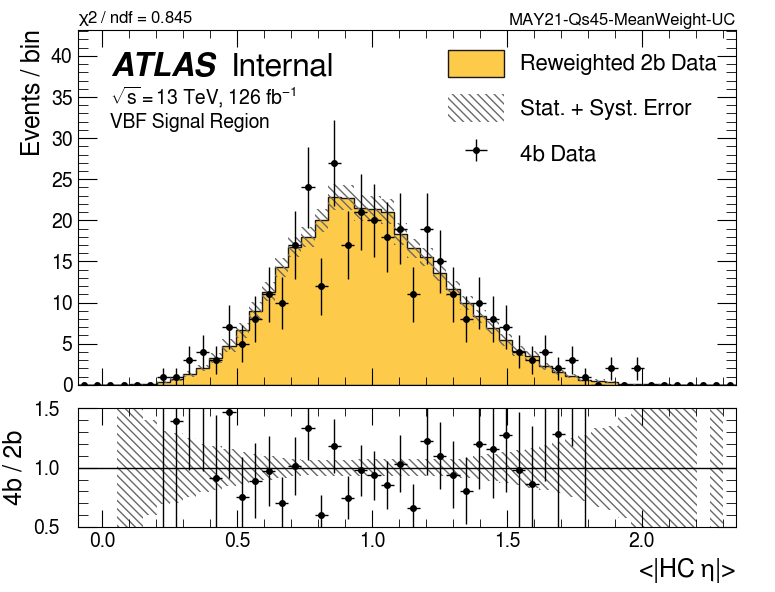
\includegraphics[width=0.25\textwidth]{\figpath{upper-center/sig/ALL/MAY21-Qs45-MeanWeight-UC-eta-i-Signal-Region-NN-all-4bvbfinclusive.png}}
    }
    \subfloat[${\pt}_{\higgs\higgs}$]{%
            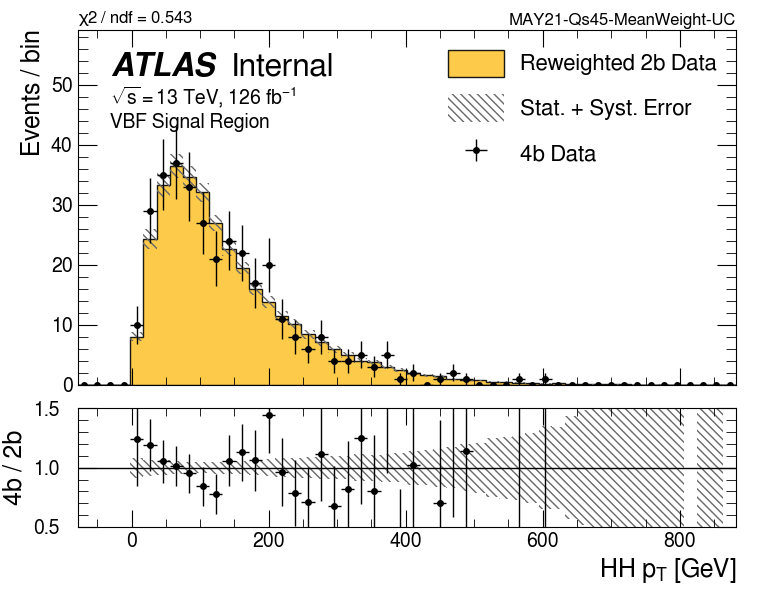
\includegraphics[width=0.25\textwidth]{\figpath{upper-center/sig/ALL/MAY21-Qs45-MeanWeight-UC-pt-hh-Signal-Region-NN-all-4bvbfinclusive.png}}
    }
    \subfloat[$dPhi_{\PH1}$]{%
            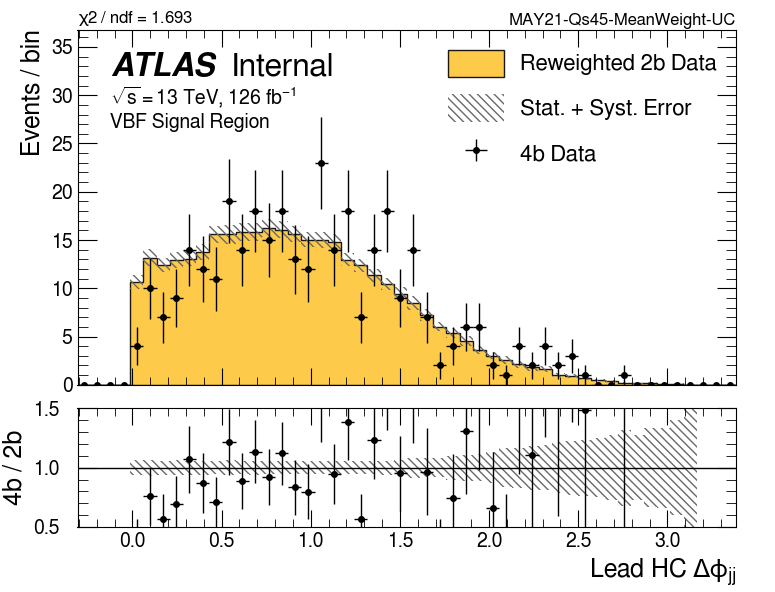
\includegraphics[width=0.25\textwidth]{\figpath{upper-center/sig/ALL/MAY21-Qs45-MeanWeight-UC-dPhi-h1-Signal-Region-NN-all-4bvbfinclusive.png}}
    }
    \subfloat[$dPhi_{\PH2}$]{%
            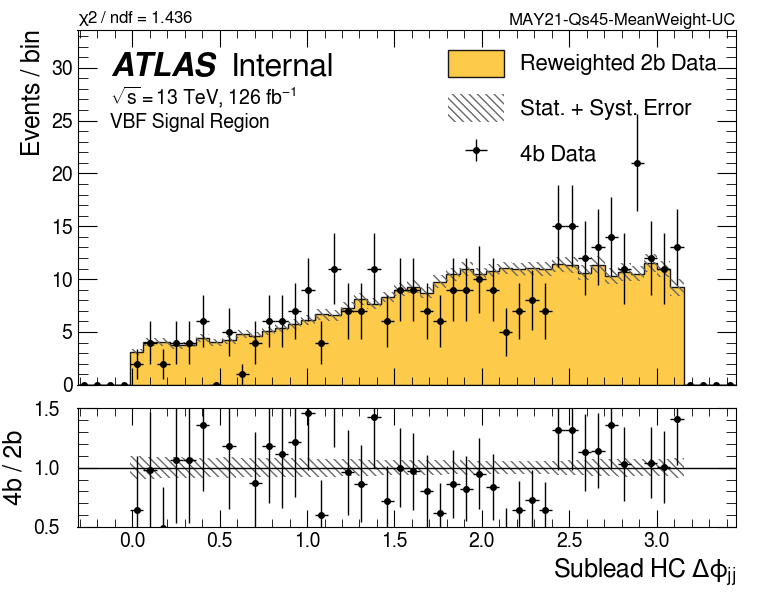
\includegraphics[width=0.25\textwidth]{\figpath{upper-center/sig/ALL/MAY21-Qs45-MeanWeight-UC-dPhi-h2-Signal-Region-NN-all-4bvbfinclusive.png}}
    }

    \subfloat[$dR_{\higgs\higgs}$]{%
            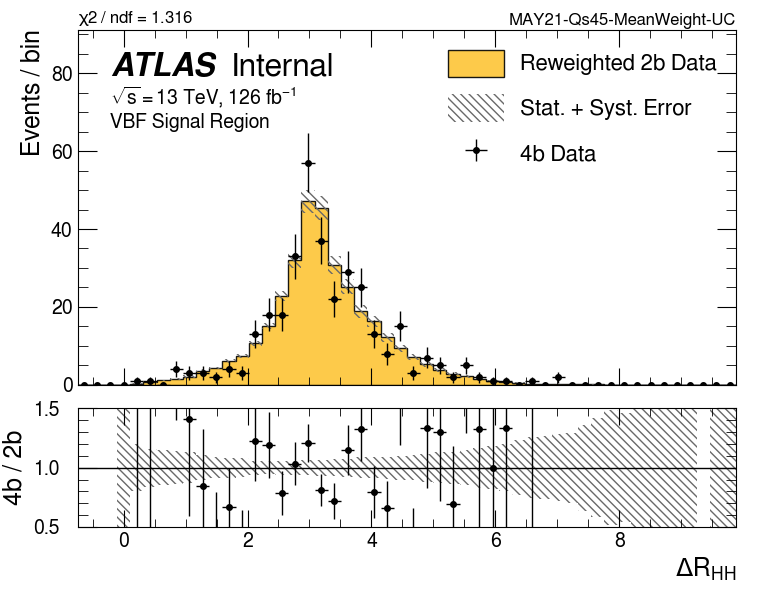
\includegraphics[width=0.25\textwidth]{\figpath{upper-center/sig/ALL/MAY21-Qs45-MeanWeight-UC-dR-hh-Signal-Region-NN-all-4bvbfinclusive.png}}
    }
    \subfloat[$dEta_{\higgs\higgs}$]{%
            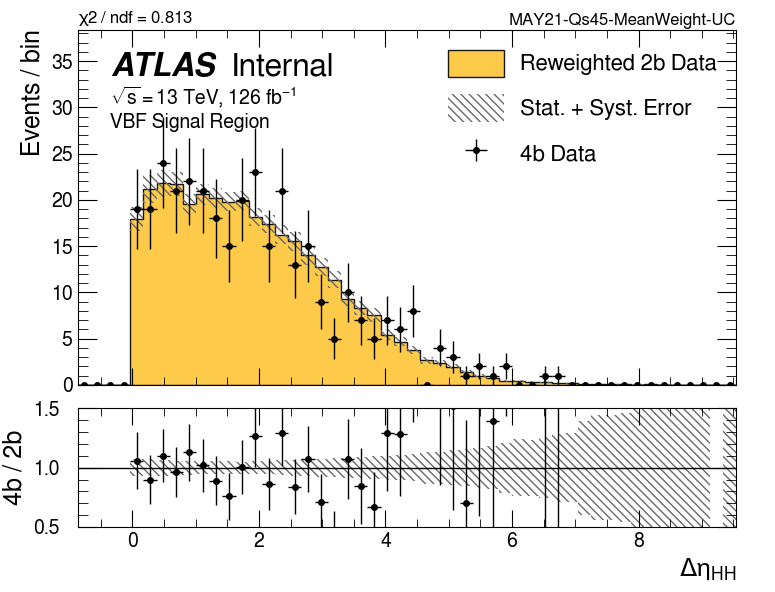
\includegraphics[width=0.25\textwidth]{\figpath{upper-center/sig/ALL/MAY21-Qs45-MeanWeight-UC-dEta-hh-Signal-Region-NN-all-4bvbfinclusive.png}}
    }
    \subfloat[$X_{wt}$]{%
            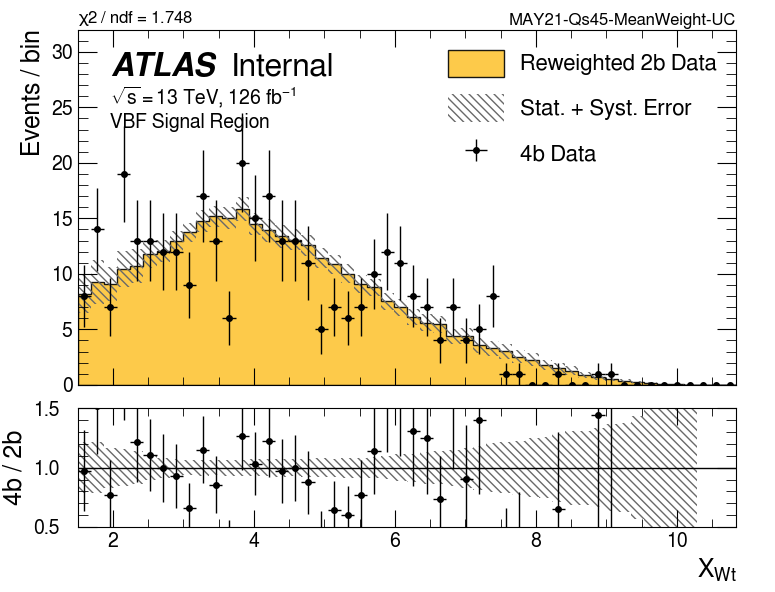
\includegraphics[width=0.25\textwidth]{\figpath{upper-center/sig/ALL/MAY21-Qs45-MeanWeight-UC-X-wt-tag-Signal-Region-NN-all-4bvbfinclusive.png}}
    }
    \subfloat[njets]{%
            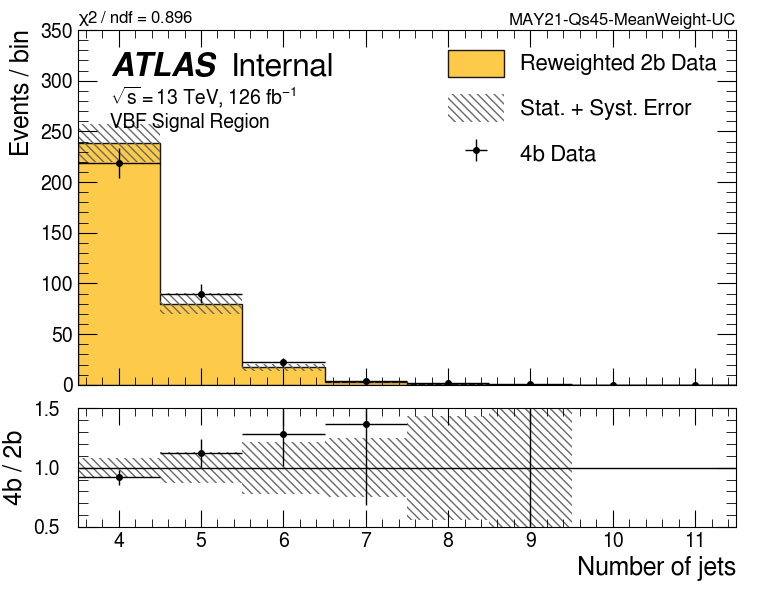
\includegraphics[width=0.25\textwidth]{\figpath{upper-center/sig/ALL/MAY21-Qs45-MeanWeight-UC-njets-Signal-Region-NN-all-4bvbfinclusive.png}}
    }

    \subfloat[${\pt}_{\PH1}$]{%
            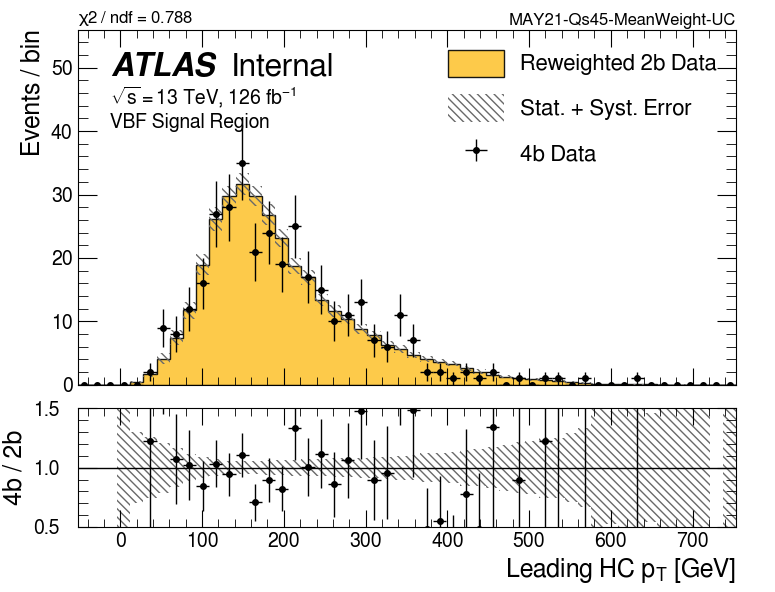
\includegraphics[width=0.25\textwidth]{\figpath{upper-center/sig/ALL/MAY21-Qs45-MeanWeight-UC-pT-h1-Signal-Region-NN-all-4bvbfinclusive.png}}
    }
    \subfloat[${\pt}_{\PH2}$]{%
            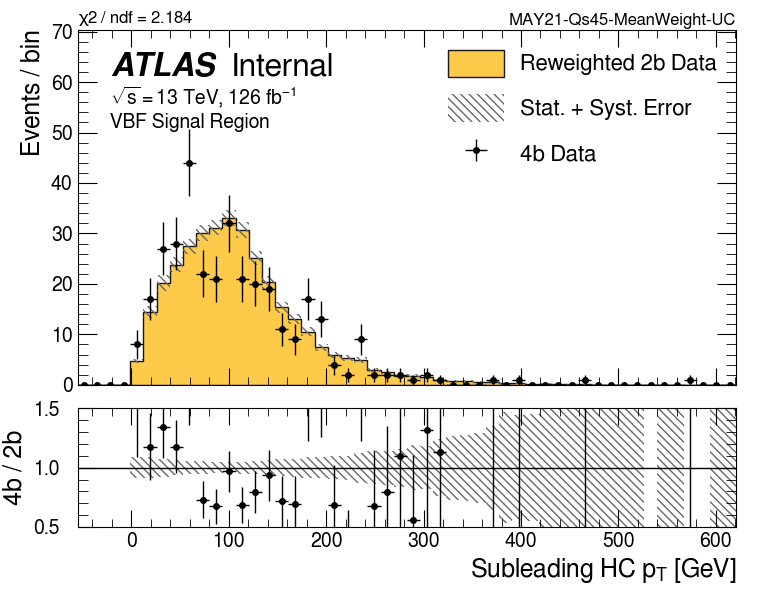
\includegraphics[width=0.25\textwidth]{\figpath{upper-center/sig/ALL/MAY21-Qs45-MeanWeight-UC-pT-h2-Signal-Region-NN-all-4bvbfinclusive.png}}
    }
    \subfloat[$m_{\PH1}$]{%
            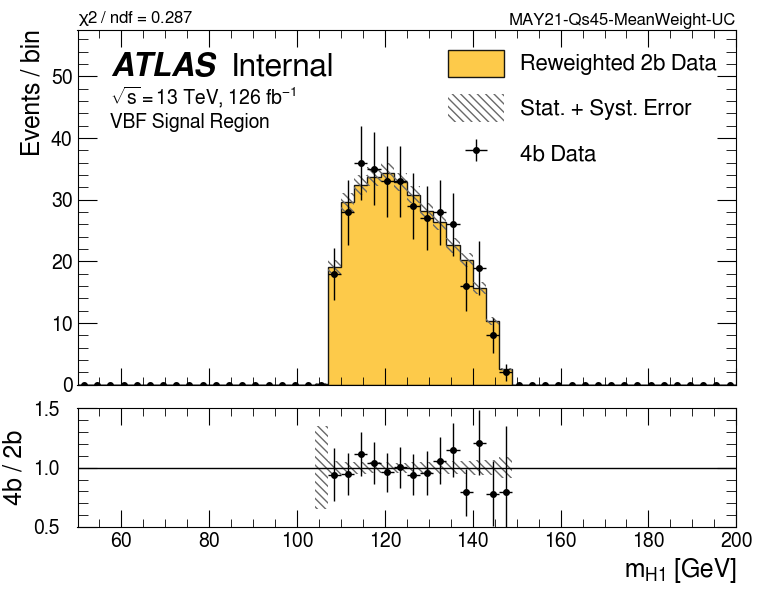
\includegraphics[width=0.25\textwidth]{\figpath{upper-center/sig/ALL/MAY21-Qs45-MeanWeight-UC-m-h1-Signal-Region-NN-all-4bvbfinclusive.png}}
    }
    \subfloat[$m_{\PH2}$]{%
            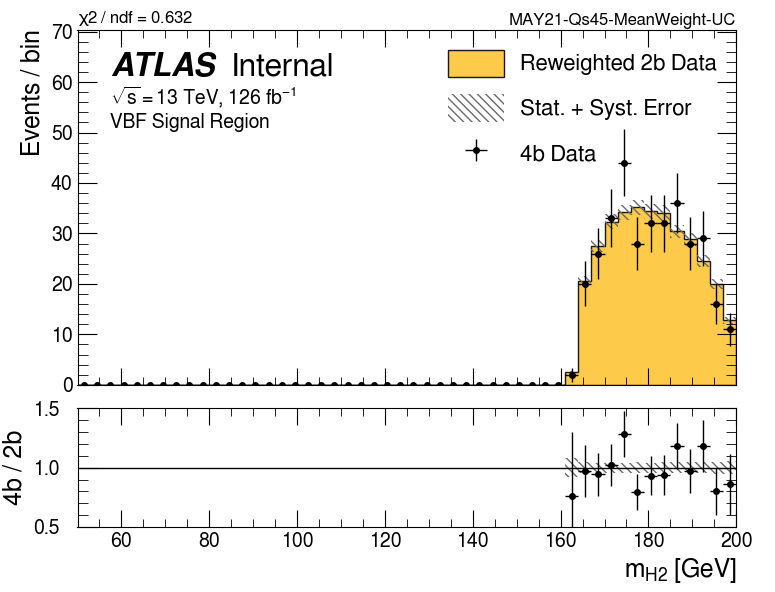
\includegraphics[width=0.25\textwidth]{\figpath{upper-center/sig/ALL/MAY21-Qs45-MeanWeight-UC-m-h2-Signal-Region-NN-all-4bvbfinclusive.png}}
    }
 
    %%%\subfloat[$\eta_{1}$]{%
    %%%        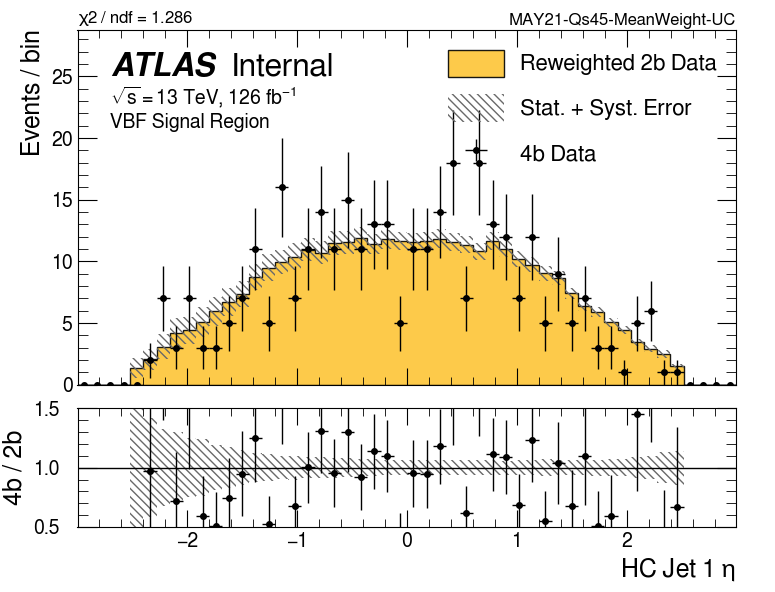
\includegraphics[width=0.25\textwidth]{\figpath{upper-center/sig/ALL/MAY21-Qs45-MeanWeight-UC-eta-1-Signal-Region-NN-all-4bvbfinclusive.png}}
    %%%}
    %%%\subfloat[$\eta_{2}$]{%
    %%%        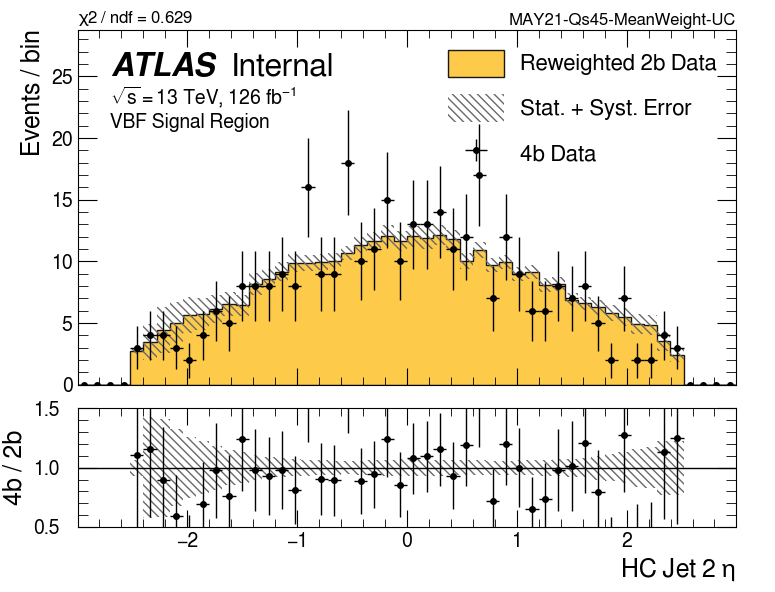
\includegraphics[width=0.25\textwidth]{\figpath{upper-center/sig/ALL/MAY21-Qs45-MeanWeight-UC-eta-2-Signal-Region-NN-all-4bvbfinclusive.png}}
    %%%}
    %%%\subfloat[$\eta_{3}$]{%
    %%%        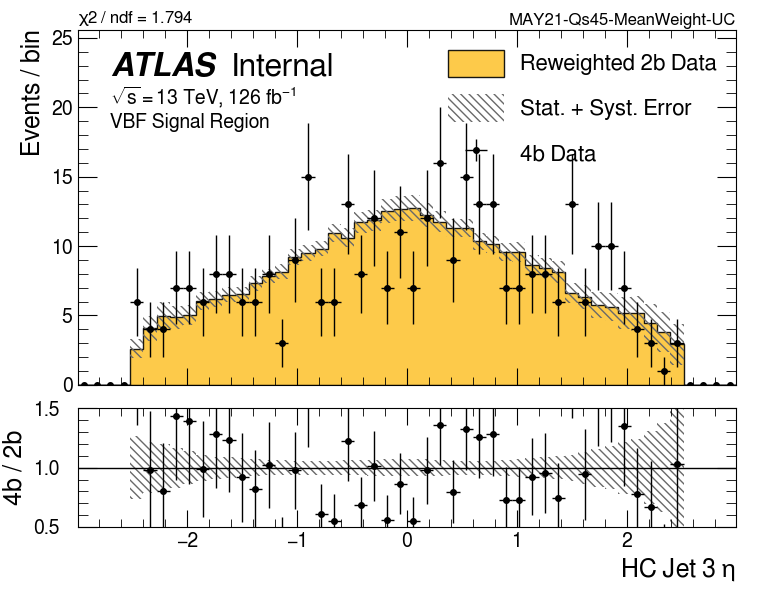
\includegraphics[width=0.25\textwidth]{\figpath{upper-center/sig/ALL/MAY21-Qs45-MeanWeight-UC-eta-3-Signal-Region-NN-all-4bvbfinclusive.png}}
    %%%}
    %%%\subfloat[$\eta_{4}$]{%
    %%%        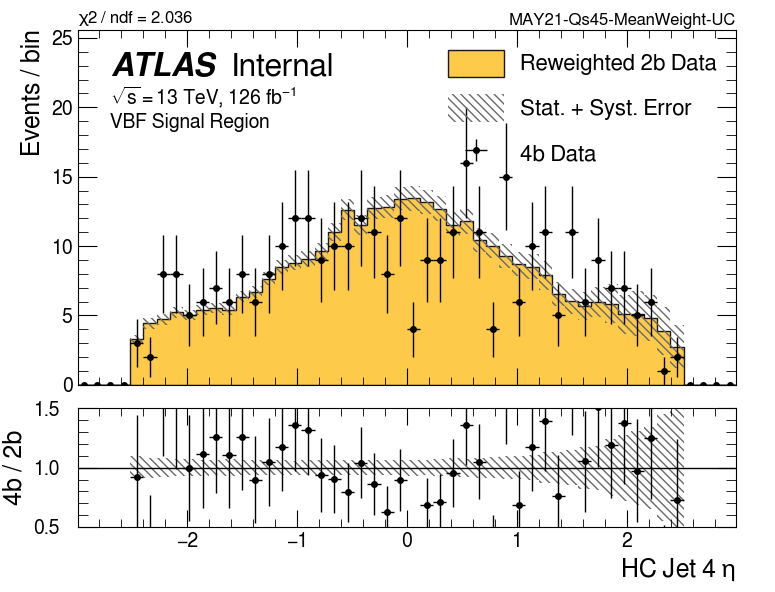
\includegraphics[width=0.25\textwidth]{\figpath{upper-center/sig/ALL/MAY21-Qs45-MeanWeight-UC-eta-4-Signal-Region-NN-all-4bvbfinclusive.png}}
    %%%}
 
    %%%\subfloat[${\pt}_{1}$]{%
    %%%        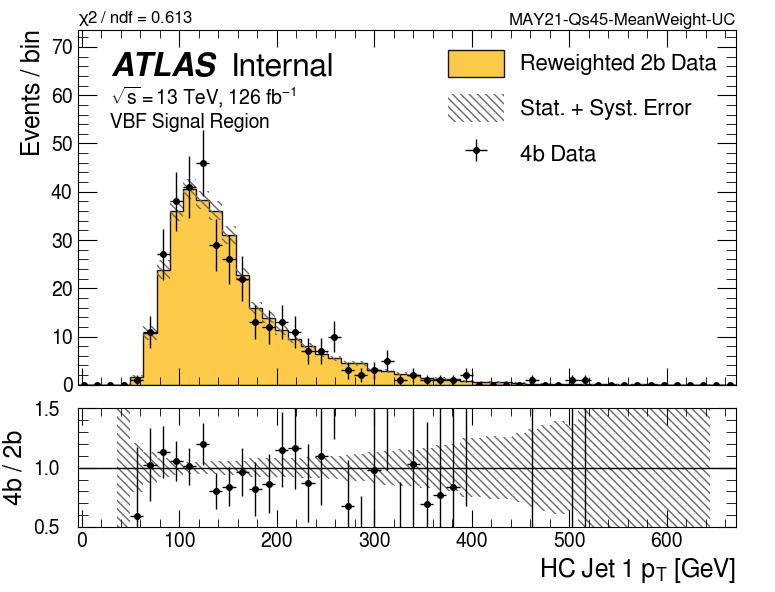
\includegraphics[width=0.25\textwidth]{\figpath{upper-center/sig/ALL/MAY21-Qs45-MeanWeight-UC-pT-1-Signal-Region-NN-all-4bvbfinclusive.png}}
    %%%}
    %%%\subfloat[${\pt}_{2}$]{%
    %%%        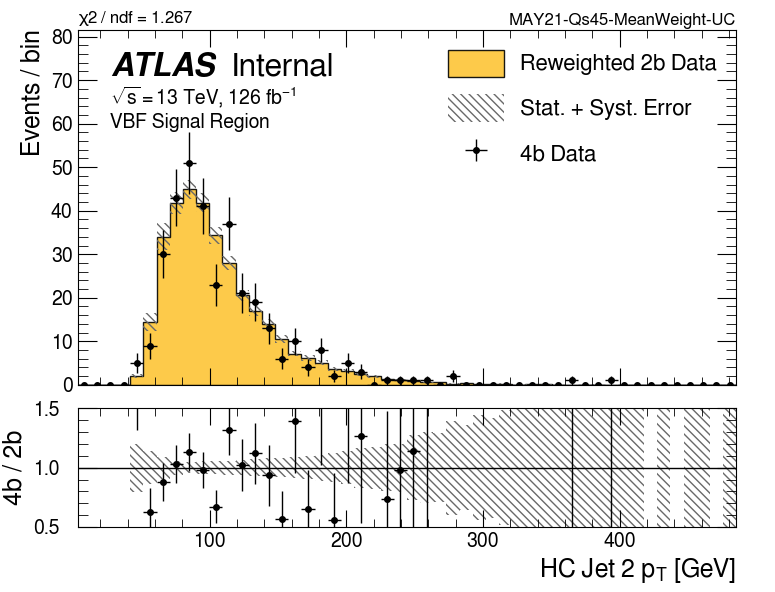
\includegraphics[width=0.25\textwidth]{\figpath{upper-center/sig/ALL/MAY21-Qs45-MeanWeight-UC-pT-2-Signal-Region-NN-all-4bvbfinclusive.png}}
    %%%}
    %%%\subfloat[${\pt}_{3}$]{%
    %%%        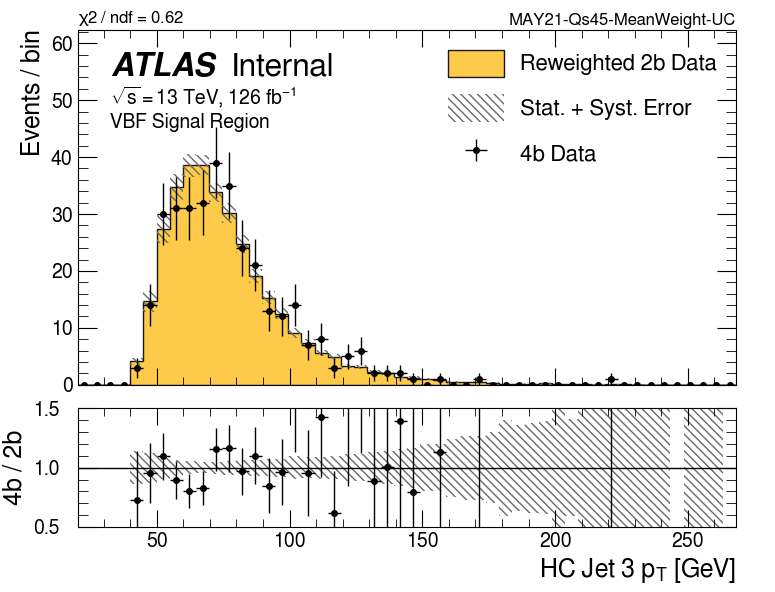
\includegraphics[width=0.25\textwidth]{\figpath{upper-center/sig/ALL/MAY21-Qs45-MeanWeight-UC-pT-3-Signal-Region-NN-all-4bvbfinclusive.png}}
    %%%}
    %%%\subfloat[${\pt}_{4}$]{%
    %%%        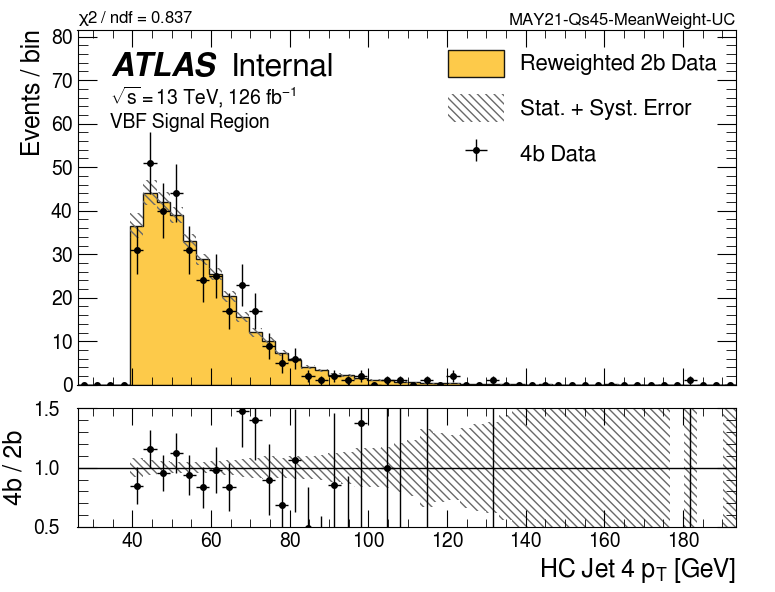
\includegraphics[width=0.25\textwidth]{\figpath{upper-center/sig/ALL/MAY21-Qs45-MeanWeight-UC-pT-4-Signal-Region-NN-all-4bvbfinclusive.png}}
    %%%}
 
    \caption{4b and reweighted 2b distributions in Signal Region in the upper center region in merged years.}
    \label{fig:upper-center-4bvbf-SR-all}
\end{figure}


